% Bounds for M_k (generated by a script).
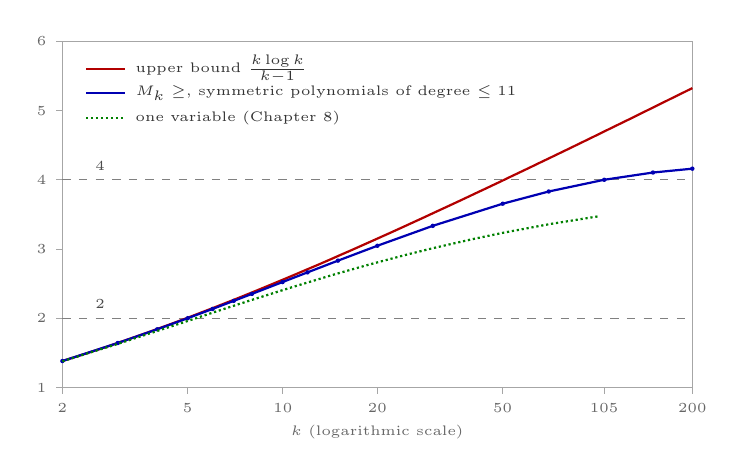
\begin{tikzpicture}[x=1cm,y=1cm]
\draw[black!35] (0,0) rectangle (8.00,4.40);
\draw[black!35] (0,0.00)--(-0.08,0.00) node[left,font=\tiny,black!60]{$1$};
\draw[black!35] (0,0.88)--(-0.08,0.88) node[left,font=\tiny,black!60]{$2$};
\draw[black!35] (0,1.76)--(-0.08,1.76) node[left,font=\tiny,black!60]{$3$};
\draw[black!35] (0,2.64)--(-0.08,2.64) node[left,font=\tiny,black!60]{$4$};
\draw[black!35] (0,3.52)--(-0.08,3.52) node[left,font=\tiny,black!60]{$5$};
\draw[black!35] (0,4.40)--(-0.08,4.40) node[left,font=\tiny,black!60]{$6$};
\draw[black!35] (0.00,0)--(0.00,-0.08) node[below,font=\tiny,black!60]{$2$};
\draw[black!35] (1.59,0)--(1.59,-0.08) node[below,font=\tiny,black!60]{$5$};
\draw[black!35] (2.80,0)--(2.80,-0.08) node[below,font=\tiny,black!60]{$10$};
\draw[black!35] (4.00,0)--(4.00,-0.08) node[below,font=\tiny,black!60]{$20$};
\draw[black!35] (5.59,0)--(5.59,-0.08) node[below,font=\tiny,black!60]{$50$};
\draw[black!35] (6.88,0)--(6.88,-0.08) node[below,font=\tiny,black!60]{$105$};
\draw[black!35] (8.00,0)--(8.00,-0.08) node[below,font=\tiny,black!60]{$200$};
\node[below,font=\tiny,black!60] at (4.00,-0.35) {$k$ (logarithmic scale)};
\draw[black!50,dashed] (0,2.64)--(8.00,2.64) node[pos=0.06,above,font=\tiny,black!70]{$4$};
\draw[black!50,dashed] (0,0.88)--(8.00,0.88) node[pos=0.06,above,font=\tiny,black!70]{$2$};
\draw[red!70!black,thick] (0.000,0.340) -- (0.101,0.372) -- (0.203,0.404) -- (0.304,0.437) -- (0.405,0.470) -- (0.506,0.503) -- (0.608,0.537) -- (0.709,0.572) -- (0.810,0.607) -- (0.911,0.642) -- (1.013,0.678) -- (1.114,0.714) -- (1.215,0.751) -- (1.316,0.788) -- (1.418,0.825) -- (1.519,0.863) -- (1.620,0.901) -- (1.722,0.940) -- (1.823,0.979) -- (1.924,1.018) -- (2.025,1.058) -- (2.127,1.098) -- (2.228,1.138) -- (2.329,1.179) -- (2.430,1.220) -- (2.532,1.262) -- (2.633,1.304) -- (2.734,1.346) -- (2.835,1.388) -- (2.937,1.431) -- (3.038,1.474) -- (3.139,1.517) -- (3.241,1.560) -- (3.342,1.604) -- (3.443,1.648) -- (3.544,1.693) -- (3.646,1.737) -- (3.747,1.782) -- (3.848,1.827) -- (3.949,1.872) -- (4.051,1.918) -- (4.152,1.963) -- (4.253,2.009) -- (4.354,2.055) -- (4.456,2.102) -- (4.557,2.148) -- (4.658,2.195) -- (4.759,2.242) -- (4.861,2.289) -- (4.962,2.336) -- (5.063,2.383) -- (5.165,2.431) -- (5.266,2.479) -- (5.367,2.526) -- (5.468,2.574) -- (5.570,2.622) -- (5.671,2.671) -- (5.772,2.719) -- (5.873,2.767) -- (5.975,2.816) -- (6.076,2.865) -- (6.177,2.913) -- (6.278,2.962) -- (6.380,3.011) -- (6.481,3.060) -- (6.582,3.109) -- (6.684,3.159) -- (6.785,3.208) -- (6.886,3.258) -- (6.987,3.307) -- (7.089,3.357) -- (7.190,3.406) -- (7.291,3.456) -- (7.392,3.506) -- (7.494,3.556) -- (7.595,3.606) -- (7.696,3.656) -- (7.797,3.706) -- (7.899,3.756) -- (8.000,3.806);
\draw[blue!70!black,thick] (0.000,0.340) -- (0.704,0.569) -- (1.204,0.743) -- (1.592,0.884) -- (1.908,1.002) -- (2.176,1.104) -- (2.408,1.193) -- (2.796,1.343) -- (3.113,1.466) -- (3.500,1.615) -- (4.000,1.804) -- (4.704,2.057) -- (5.592,2.338) -- (6.176,2.493) -- (6.881,2.642) -- (7.500,2.734) -- (8.000,2.783);
\fill[blue!70!black] (0.000,0.340) circle (0.8pt);
\fill[blue!70!black] (0.704,0.569) circle (0.8pt);
\fill[blue!70!black] (1.204,0.743) circle (0.8pt);
\fill[blue!70!black] (1.592,0.884) circle (0.8pt);
\fill[blue!70!black] (1.908,1.002) circle (0.8pt);
\fill[blue!70!black] (2.176,1.104) circle (0.8pt);
\fill[blue!70!black] (2.408,1.193) circle (0.8pt);
\fill[blue!70!black] (2.796,1.343) circle (0.8pt);
\fill[blue!70!black] (3.113,1.466) circle (0.8pt);
\fill[blue!70!black] (3.500,1.615) circle (0.8pt);
\fill[blue!70!black] (4.000,1.804) circle (0.8pt);
\fill[blue!70!black] (4.704,2.057) circle (0.8pt);
\fill[blue!70!black] (5.592,2.338) circle (0.8pt);
\fill[blue!70!black] (6.176,2.493) circle (0.8pt);
\fill[blue!70!black] (6.881,2.642) circle (0.8pt);
\fill[blue!70!black] (7.500,2.734) circle (0.8pt);
\fill[blue!70!black] (8.000,2.783) circle (0.8pt);
\draw[green!50!black,thick,densely dotted] (0.000,0.337) -- (0.704,0.558) -- (1.204,0.722) -- (1.592,0.849) -- (1.908,0.954) -- (2.176,1.042) -- (2.408,1.117) -- (2.613,1.182) -- (2.796,1.240) -- (2.961,1.291) -- (3.113,1.337) -- (3.252,1.379) -- (3.380,1.418) -- (3.500,1.453) -- (3.612,1.485) -- (3.718,1.515) -- (3.817,1.543) -- (3.911,1.569) -- (4.000,1.593) -- (4.388,1.695) -- (4.704,1.773) -- (5.204,1.887) -- (5.592,1.968) -- (6.176,2.077) -- (6.796,2.176);
\draw[red!70!black,thick] (0.30,4.05)--(0.80,4.05) node[right,font=\tiny,black!80]{upper bound $\frac{k\log k}{k-1}$};
\draw[blue!70!black,thick] (0.30,3.74)--(0.80,3.74) node[right,font=\tiny,black!80]{$M_k\ge$, symmetric polynomials of degree $\le11$};
\draw[green!50!black,thick,densely dotted] (0.30,3.43)--(0.80,3.43) node[right,font=\tiny,black!80]{one variable (Chapter 8)};
\end{tikzpicture}
